\section{Reviewer's question}
\subsection*{Reviewer's question}

\begin{frame}
\begin{block}{Question}
\begin{otherlanguage}{czech}
Zkoušel jste filtr testovat na scénáři kde je cíl vidět na počátku trajektorie, avšak poté ztratíme velké množství měření? Dokáže filtr tuto situaci vyřešit, nebo pro něj půjde o nově vzniklý objekt, který nevznikl v očekávané oblasti a nebude tedy sledován?
\end{otherlanguage}
\end{block}
\begin{exampleblock}{Answer}
\begin{itemize}
    \item Při nastavení $P_{D,k}=0.7$, což znamená, že průměrně 30\% měření rovnoměrně v čase je ztraceno, filtr dokázal tyto misdetekce správně vyřešit.
    \item Nový scénář: Dva objekty generují měření po dobu 45 kroků, poté 10 kroků pauza, pak se 45 kroků měření znovu generují.
    \item Filtr ztrácí sledování objektů již po několika krocích bez měření a pozdější měření nedokáže odlišit od šumu.
    \item \textbf{Odpověď:} Pro filtr se jedná o nově vzniklý objekt v neočekávané oblasti, který nakonec nebude sledován.
\end{itemize}
\end{exampleblock}
\end{frame}

\begin{frame}
\begin{columns}
    \begin{column}{0.5\textwidth}
        \begin{figure}[ht]
            \centering
            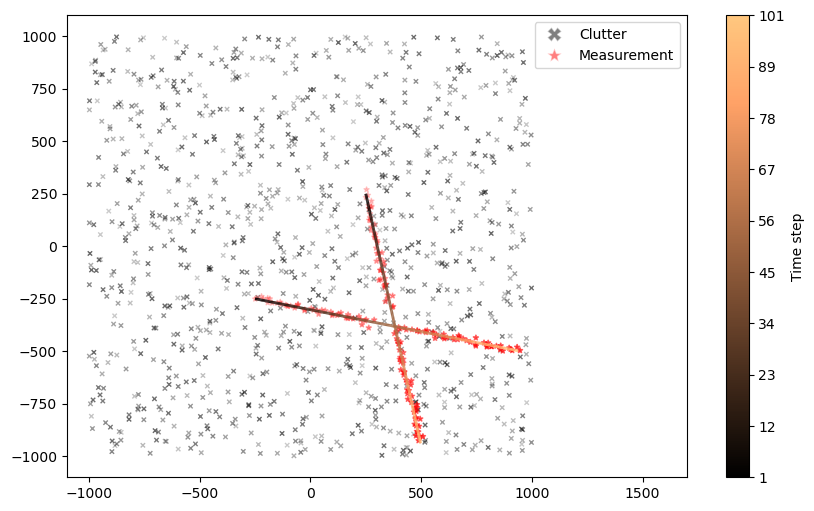
\includegraphics[width=\linewidth]{pic/review-meas.png}
            \caption{True measurements and clutter.}
        \end{figure}
    \end{column}
    \begin{column}{0.5\textwidth}
        \begin{figure}[ht]
            \centering
            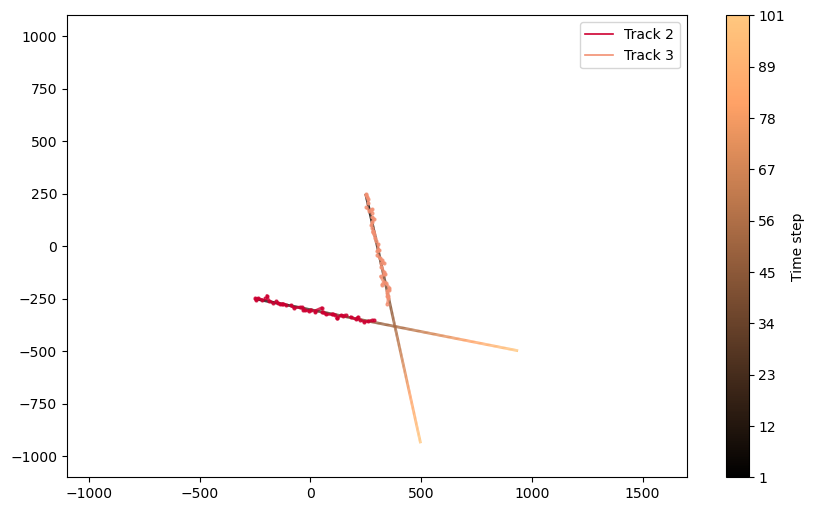
\includegraphics[width=\linewidth]{pic/review-est.png}
            \caption{Tracks are terminated soon after measurements are gone.}
        \end{figure}
    \end{column}
\end{columns}
\end{frame}

\begin{frame}
    \transduration<1->{0.3}
    \centering
    \multiinclude[<+->][format=png, graphics={width=0.8\linewidth}, start=1]{pic/posterior/posterior}
\end{frame}
